
%%%%%%%%%%%%%%%%%%%%%%%%%%%%%%%%%%%%%%%%%%%%%%%%%%%%%%%%%%%%%%%%%%%%%
%% This is a (brief) model paper using the achemso class
%% The document class accepts keyval options, which should include
%% the target journal and optionally the manuscript type.
%%%%%%%%%%%%%%%%%%%%%%%%%%%%%%%%%%%%%%%%%%%%%%%%%%%%%%%%%%%%%%%%%%%%%
\documentclass[journal=jctcce,manuscript=article]{achemso}

%%%%%%%%%%%%%%%%%%%%%%%%%%%%%%%%%%%%%%%%%%%%%%%%%%%%%%%%%%%%%%%%%%%%%
%% Place any additional packages needed here.  Only include packages
%% which are essential, to avoid problems later. Do NOT use any
%% packages which require e-TeX (for example etoolbox): the e-TeX
%% extensions are not currently available on the ACS conversion
%% servers.
%%%%%%%%%%%%%%%%%%%%%%%%%%%%%%%%%%%%%%%%%%%%%%%%%%%%%%%%%%%%%%%%%%%%%
\usepackage[version=3]{mhchem} % Formula subscripts using \ce{}
\usepackage[T1]{fontenc}       % Use modern font encodings
\usepackage{amsmath}	    % American Mathematical Society equation formatting
\graphicspath{ {images/} }     % Path to images
%TO REMOVE BEFORE SUBMISSION
\usepackage{lineno} % add the line numbers
\linenumbers
%END TO REMOVE BEFORE SUBMISSION

%%%%%%%%%%%%%%%%%%%%%%%%%%%%%%%%%%%%%%%%%%%%%%%%%%%%%%%%%%%%%%%%%%%%%
%% If issues arise when submitting your manuscript, you may want to
%% un-comment the next line.  This provides information on the
%% version of every file you have used.
%%%%%%%%%%%%%%%%%%%%%%%%%%%%%%%%%%%%%%%%%%%%%%%%%%%%%%%%%%%%%%%%%%%%%
%%\listfiles

%%%%%%%%%%%%%%%%%%%%%%%%%%%%%%%%%%%%%%%%%%%%%%%%%%%%%%%%%%%%%%%%%%%%%
%% Place any additional macros here.  Please use \newcommand* where
%% possible, and avoid layout-changing macros (which are not used
%% when typesetting).
%%%%%%%%%%%%%%%%%%%%%%%%%%%%%%%%%%%%%%%%%%%%%%%%%%%%%%%%%%%%%%%%%%%%%
\newcommand*\mycommand[1]{\texttt{\emph{#1}}}

%%%%%%%%%%%%%%%%%%%%%%%%%%%%%%%%%%%%%%%%%%%%%%%%%%%%%%%%%%%%%%%%%%%%%
%% Meta-data block
%% ---------------
%% Each author should be given as a separate \author command.
%%
%% Corresponding authors should have an e-mail given after the author
%% name as an \email command. Phone and fax numbers can be given
%% using \phone and \fax, respectively; this information is optional.
%%
%% The affiliation of authors is given after the authors; each
%% \affiliation command applies to all preceding authors not already
%% assigned an affiliation.
%%
%% The affiliation takes an option argument for the short name.  This
%% will typically be something like "University of Somewhere".
%%
%% The \altaffiliation macro should be used for new address, etc.
%% On the other hand, \alsoaffiliation is used on a per author basis
%% when authors are associated with multiple institutions.
%%%%%%%%%%%%%%%%%%%%%%%%%%%%%%%%%%%%%%%%%%%%%%%%%%%%%%%%%%%%%%%%%%%%%
\author{Alexander Punter}
\author{Paola Nava}
\author{Yannick Carissan}
\email{Yannick.Carissan@univ-amu.fr}
\phone{+33 (0)491289168}
\affiliation[Aix-Marseille University]
{Aix Marseille Univ, CNRS, Centrale Marseille, iSm2, Marseille, France}
%%%%%%%%%%%%%%%%%%%%%%%%%%%%%%%%%%%%%%%%%%%%%%%%%%%%%%%%%%%%%%%%%%%%%
%% The document title should be given as usual. Some journals require
%% a running title from the author: this should be supplied as an
%% optional argument to \title.
%%%%%%%%%%%%%%%%%%%%%%%%%%%%%%%%%%%%%%%%%%%%%%%%%%%%%%%%%%%%%%%%%%%%%
\title[A great title]
  {A great title}

%%%%%%%%%%%%%%%%%%%%%%%%%%%%%%%%%%%%%%%%%%%%%%%%%%%%%%%%%%%%%%%%%%%%%
%% Some journals require a list of abbreviations or keywords to be
%% supplied. These should be set up here, and will be printed after
%% the title and author information, if needed.
%%%%%%%%%%%%%%%%%%%%%%%%%%%%%%%%%%%%%%%%%%%%%%%%%%%%%%%%%%%%%%%%%%%%%
\abbreviations{IR,NMR,UV}
\keywords{Pseudo-potentials, Group potentials}

%%%%%%%%%%%%%%%%%%%%%%%%%%%%%%%%%%%%%%%%%%%%%%%%%%%%%%%%%%%%%%%%%%%%%
%% The manuscript does not need to include \maketitle, which is
%% executed automatically.
%%%%%%%%%%%%%%%%%%%%%%%%%%%%%%%%%%%%%%%%%%%%%%%%%%%%%%%%%%%%%%%%%%%%%
\begin{document}

%%%%%%%%%%%%%%%%%%%%%%%%%%%%%%%%%%%%%%%%%%%%%%%%%%%%%%%%%%%%%%%%%%%%%
%% The "tocentry" environment can be used to create an entry for the
%% graphical table of contents. It is given here as some journals
%% require that it is printed as part of the abstract page. It will
%% be automatically moved as appropriate.
%%%%%%%%%%%%%%%%%%%%%%%%%%%%%%%%%%%%%%%%%%%%%%%%%%%%%%%%%%%%%%%%%%%%%
\begin{tocentry}

Some journals require a graphical entry for the Table of Contents.
This should be laid out ``print ready'' so that the sizing of the
text is correct.

Inside the \texttt{tocentry} environment, the font used is Helvetica
8\,pt, as required by \emph{Journal of the American Chemical
Society}.

The surrounding frame is 9\,cm by 3.5\,cm, which is the maximum
permitted for  \emph{Journal of the American Chemical Society}
graphical table of content entries. The box will not resize if the
content is too big: instead it will overflow the edge of the box.

This box and the associated title will always be printed on a
separate page at the end of the document.

\end{tocentry}

%%%%%%%%%%%%%%%%%%%%%%%%%%%%%%%%%%%%%%%%%%%%%%%%%%%%%%%%%%%%%%%%%%%%%
%% The abstract environment will automatically gobble the contents
%% if an abstract is not used by the target journal.
%%%%%%%%%%%%%%%%%%%%%%%%%%%%%%%%%%%%%%%%%%%%%%%%%%%%%%%%%%%%%%%%%%%%%
\begin{abstract}
A pseudo-potential system for recreating an sp\(^{2}\) carbon atom is built 
and tested as a building block for various pseudo-hydrocarbon chain and ring systems.  
This pseudo-system has a central charge of 1, thus it contains only one
electron. It has been employed in \textsl{ab-initio} calculations:
1\textsuperscript{st} ionisation and excitation energies, as well as the HOMO energy, 
are found to be reproduced to a good accuracy by the pseudo-system.
\end{abstract}

%%%%%%%%%%%%%%%%%%%%%%%%%%%%%%%%%%%%%%%%%%%%%%%%%%%%%%%%%%%%%%%%%%%%%
%% Start the main part of the manuscript here.
%%%%%%%%%%%%%%%%%%%%%%%%%%%%%%%%%%%%%%%%%%%%%%%%%%%%%%%%%%%%%%%%%%%%%
\section{Introduction}

\newcounter{customItem}
\newcommand{\showCustomItem}{\refstepcounter{customItem}\roman{customItem}}

%For most of the quantum chemistry calculations, the system can be divided into two parts:
%the active part, \emph{i.e.} the part of the molecule one is interested in and
%the inactive part, which is to be taken into account in order to fulfill chemical requirements.
It is a common idea that a chemical system can be thought of as comprised of (at least) 
two parts:
an active one, where most of the chemistry takes place, and an (apparently) inactive
one, which must be taken into account in order to fulfill chemical requirements.
Based on this general statement, many successful theoretical approaches have been developed.
Among them can be cited QM/QM' or QM/MM methods (\showCustomItem), where 
the active region that usually contains several atoms is
treated at a high level of calculation, while the inactive part is treated at a 
lower level of theory.\cite{chung_oniom_2015}
Frozen density embedding techniques (\showCustomItem) replace part of a molecule, or 
its surroundings,
by a frozen electronic density extracted on a reference system.\cite{wesolowski_frozen-density_2015}
They are an extension of the frozen core approximation, already used %in the early days 
to reduce
the number of parameters to be optimized in the self consistent field calculation.

In this article we shall focus on pseudo-potential techniques, which also
divide the chemical problem into two parts.
Effective core potentials (\showCustomItem) are commonly employed for atoms: 
core electrons (and effects due to the corresponding nuclear charge) are
replaced by an operator fast to evaluate and the active electrons are treated
explicitly.\cite{dolg_relativistic_2012}
In the same vein, model potentials (\showCustomItem) replace a frozen electronic density (computed from the atom)
by some operators, the number of which depends on the level of
refinement required.\cite{huzinaga_1994_1995}

The effective group potentials (\showCustomItem) bridge the frozen density and the core potential
approaches: using core potential extraction techniques, effects due to the implicit 
electron density (and corresponding nuclear charge) 
are reproduced by a mono-electronic operator.\cite{carissan_what_2006}
However, while effective core potentials and model potentials intend to 
reproduce atomic properties,
effective group potentials aim at mimicking the effect of atoms involved in one or more chemical
bonds. The cyclopentadienyl group has, for instance, been successfully extracted.
In this example, the active part consisted of six electrons (the $\pi$ electrons) and six
nuclear charges, with the pseudo-potential replacing all the rest, including the hydrogen atoms.
Even if the $\sigma / \pi$ separability suggested how to define the active and the inactive parts,
carbon atoms are hybridized and the core/valence distinction is not 
strictly defined.

The theoretical background to extract effective group pseudo-potentials  can be traced back 
to several contributions in the 80's and 90's. In 1985 Katsuki built molecular potentials based on Huzinaga's model potentials.
 In his work on this subject, Huzinaga emphasises that pseudo-potentials should maintain three effects of the
'dormant' electrons on the active ones: the Coulomb, the exchange and the 'no-collapse' term.\cite{huzinaga_effective_1991}
Following his proposal, for an atom where active and dormant electrons have been separated, the Hamiltonian reads:
\begin{equation}
\label{eq:atomicHamiltonian}
\hat{H} = \sum_{i=1}^n \hat{h}(i) +\sum_{i<j}\frac{1}{r_{ij}}
\end{equation}
with $\frac{1}{r_{ij}}$ the bielectronic interaction
between explicitly treated active electrons and
the mono-electronic operator:
\begin{equation}
\label{eq:monoElectronicOperator}
\hat{h}(i) = -\frac{1}{2}\Delta_i - \frac{(Z-Z_c)}{r_i}+\hat{V}(i) + \hat{\sigma}(i)
\end{equation}
where $\Delta_i$ is the Laplacian of the coordinates of electron $i$, and 
$Z_C$ is the number of core electrons withdrawn from the reference system.
The operator $\hat{\sigma}(i)$ is the 'no-collapse' term that prevents active electrons
collapsing into the dormant region. The operator $\hat{V}(i)$ reproduces the 
Coulomb and exchange interactions, for which Hunzinaga proposed a spectral formulation:
\begin{equation}
\label{eq:HuzinagaMPVersion1Potential}
\hat{V} = r^{-n}\left[\sum_IA_I\exp(-\alpha_I r^2)+\sum_JB_Jr\exp(-\beta_J r^2)\right] \text{with}\;n=1
\end{equation}

To take into account the fact that dormant electrons are removed from the
system, the nuclear charge is modified by the $Z_c$ value.
Yet, as the effective charge felt by the active electrons is likely not to be an integer,
the modification of the value of the nuclear charge is scaled in $\hat{V}$.
In this operator we notice that the \(r^{-1}\) behavior is mantained for the first term 
(the Coulomb one).

%Let us follow Huzinaga in his enlightening work.\cite{huzinaga_effective_1991}
%In order to extract a meaningful potential, he states that for electron/electron interactions, 
%"the most important effect is that the exclusion principle prevents active electrons
%from collapsing into the dormant region.
%The second is the exchange energy terms between the dormant and active electrons
%through their electrostatic interaction."
%For an atom, the Hamiltonian reads:
%\begin{equation}
%\label{eq:atomicHamiltonian}
%\hat{H} = \sum_{i=1}^n \hat{h}(i) +\sum_{i<j}\frac{1}{r_{ij}}
%\end{equation}
%with $\frac{1}{r_{ij}}$ the bielectronic interaction
%between explicitly treated active electrons and
%the mono electronic operator:
%\begin{equation}
%\label{eq:monoElectronicOperator}
%\hat{h}(i) = -\frac{1}{2}\Delta_i - \frac{(Z-Z_c)}{r_i}+\hat{V}(i) + \hat{\sigma}(i)
%\end{equation}
%where
%$\Delta_i$ is the laplacian of the coordinates of electron $i$,
%$Z_C$ is the number of core electrons withdrawn from the reference system,
%$\hat{V}(i)$ the pseudo-potential which reproduces the electrostatic
%interaction between the dormant and active electrons
%and $\hat{\sigma}(i)$ the operator, which models the exclusion principle
%and prevents active electrons from collapsing into the dormant region.
%To take into account the fact that dormant electrons are removed from the
%system, the nuclear charge is modified by the $Z_c$ value.
%Yet, as the effective charge felt by the active electrons is likely not to be an integer,
%the modification of the value of the nuclear charge is scaled in $\hat{V}$.
%Depending on the version used, this modification differs.
%In this work, we take as a reference version 1 as defined in
%Huzinaga's lecture\cite{huzinaga_1994_1995}:
%\begin{equation}
%\label{eq:HuzinagaMPVersion1Potential}
%\hat{V} = \frac{1}{r}\left[\sum_IA_I\exp(-\alpha r^2)+\sum_JB_Jr\exp(-\beta r^2)\right]
%\end{equation}
%In this model potential version, $\hat{\sigma}$ is defined as:
%\begin{equation}
%\label{eq:HuzinagaMPVersion1Sigma}
%\hat{\sigma} = -\sum f_c\epsilon_c\left|\phi_c\right>\left<\phi_c\right|
%\end{equation}
%with $\epsilon_c$ the eigenvalue of the core orbital $\phi_c$ and
%$f_c$ an optimized parameter.
%In the other versions of model potentials, $f_c=2$, as suggested earlier.\cite{houjer_aspects_1978}

%In the present work, we shall optimize the parameters in $\hat{V}$ and $\hat{\sigma}$
%for hybridized atoms.
%Before going further, it is important to stress that hybridization implies that the
%$\left\{\phi_c\right\}_i$ are linear combination of atomic orbitals and that
%$\hat{V}$ should no more be spherical.
%This loss of isotropy combined with the loss of clear core/valence separation
%will imply constraints during the extraction process.

In the present work, the aim is not to obtain pseudo-potentials for  specific
chemical groups, as in the case of the cyclopentadienyl anion cited hereabove.
Instead, we want to propose a methodology for extracting a potential for
a hybridised carbon atom (here an $sp^2$ carbon atom), which can then be
used as a building block for constructing chemical systems. This carbon atom
will contain explicitly one nuclear charge and one electron.
Moreover, the method should be usable 
%In this work, we aim at developing a method usable 
out of the box in any standard quantum chemistry software.
Thus, no modification of the source code should be done.
This supplementary constraint will be fulfilled by strategically positioning the pseudo-potentials
we intend to use. 

Pseudo-potentials for hybridised carbon
atoms have been already successfully extracted in a previous work of ours.\cite{drujon_pseudopotentials_2013}
There, our attention was focused on the 'no-collapse' term, and 
functions in the pseudo-potential shift up unwanted orbitals and correctly place the energy of the
wanted orbitals.
%However, in our extraction procedure, some pseudo-potentials had to be put precisely at the center
%of each bond.
However, some pseudo-potentials had to be put precisely at the center
of each bond.
Thus, those pseudo-potentials could not be considered as atomic as they were not defined solely
with respect to the position of the atom they applied to. The previous work should therefore be regarded as a proof-of-concept.
In this new version, we include more physical meaning in our model, 
by placing pseudo-potentials that mimic Coulomb interactions among the active and dormant electrons, and the shielded nuclear charge. 
The new pseudo-potentials are fully atomic: the position of the atom
determines completely where the potentials are put in space in the best possible manner
when dealing with hybridized atoms (as hybridization destroys isotropy, the preferred orientations
must be given to define the pseudo-potential).

This article is structured as follows.
In the first part, the method is defined in detail.
The second part shows the results obtained, from the most crude to the most refined
version of the method.
The extracted pseudopotentials are then employed for extended systems.
Perspectives are presented in the conclusion.

\section{Method}

\subsection{Pseudopotential definition}

As in our previous work\cite{drujon_pseudopotentials_2013},
we take CH\(^{\bullet}_{3}\) as our starting system to be reproduced.
It is the smallest system containing one and only one sp$^2$ hybridized carbon atom.
This choice allows us to isolate the different electrostatic interactions
to build a physically meaningful model.
%In order to fulfil the criteria specified in Equation (\ref{eq:atomicHamiltonian}),
We make use of two kinds of Gaussian pseudo-potentials \cite{me_structure_theory}, of \(s\) and \(p\) shapes. As we want to avoid modifying the quantum chemistry software itself, the pseudo-potentials have a semi-local form and we choose a value of \(n = 1\) to preserve the \(r^{-1}\) behaviour as in Huzinaga's work.
The multi-centered pseudo-potentials that we build read as follows:
\begin{equation}
\label{eq:ourPP}
\hat{W} = r^{-n}\left[%
\underbrace{\sum_IA_I\exp(-\alpha_I r^2)\left|Y_{1,m}\right>\left<Y_{1,m}\right|}_{\text{p projectors}}%
+%
\underbrace{\sum_JC_Jr\exp(-\gamma_J (r-r^0_J)^2)\left|Y_{0,0}\right>\left<Y_{0,0}\right|}_{\text{s projectors}}%
\right]
\end{equation}
with $Y_{0,0}$ the $s$ spherical harmonic, $Y_{1,m}$ the $p$ spherical harmonics (the sum over $m$
is not written explicitly to improve readability) and $r^0_J$ the relative fixed position of the $J^{th}$
potential with respect to the origin of the pseudo-atom, which carries the pseudo-potentials.
By analogy with Huzinaga model potentials defined in (\ref{eq:HuzinagaMPVersion1Potential})
we can say that the $p$ projectors aim to mimic a coulombic interaction,
while the $s$ potentials have the task of recovering part of the bi-electronic interaction
between the dormant and the active electrons.
Thus, this second term is not stricly equivalent to Huzinaga's $B_J$ terms as they aim at recovering
the bi-eletronic interactions and the no-collapse term.
This later role was devoted to the $\hat{\sigma}$ operator in Huzinaga's formulation.

As will be discussed in the following sections,
the \(p\) pseudo-potential allows to reproduce atomic properties, when the
\(s\)-potentials mimic electrostatic electron pair repulsion. The pseudo-potentials are mono-electronic operators, thus they shall not be able to reproduce fully bi-electronic interactions. Knowing this, we adjust the parameters of the \(s\)-potentials for the pseudo-system to have a wavefunction in which properties, such as spatial extent, energy and excitation energies, are as close as possible to those of the reference system.

\begin{figure}[ht]
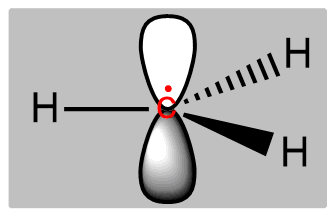
\includegraphics[width=8cm]{ch3.png}
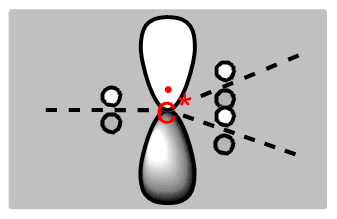
\includegraphics[width=8cm]{pseudoch3.png}
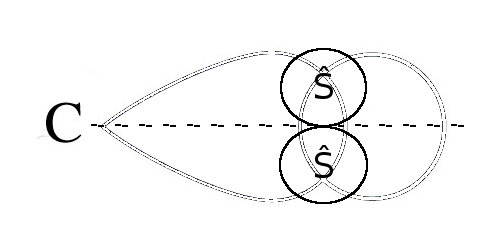
\includegraphics[width=8cm]{tm_sp2_potentials.png}
\caption{Diagrams of CH\(^{\bullet}_{3}\) (left) and pseudo-CH\(^{\bullet}_{3}\) (right, below) molecules. The pseudo-CH\(^{\bullet}_{3}\) diagrams display the \(s\) and \(p\)-potential positions, and the distances \(d\) and \(c\).}
\label{figure:ref_pseudo_diagram}
\end{figure}

Figure \ref{figure:ref_pseudo_diagram} displays the final pseudo-system: The CH\(^{\bullet}_{3}\) radical has been replaced by
a hydrogen-like "pseudo-carbon", with a nuclear charge of \(Z_{nucleus} = 1\), and one electron occupying the \(p_{z}\) orbital. 
There are now no H atoms, and the system is surrounded by three potential sets at a planar distance of \(d\), each consisting of 
two \(s\)-shaped potentials with a distance above and below the \(xy\)-plane of \(c\). A further \(p\)-shaped potential is applied
directly to the pseudo-carbon.

This gives multiple variables we can use to manipulate the properties of the system.
We can alter the strength and diffuseness of the \(p\) and \(s\) potentials themselves,
as well as vary the distances \(d\) and \(c\) by moving the \(s\)-potentials.
In this article, we fix \(c = 0.25\;a.u.\).

\subsection{Making Potentials Physically Meaningful}
\label{section:potential_derivation}

It is possible to obtain the potential parameters entirely by empirical means, in principle. However, we can make a more informed guess at some starting parameters from which to optimise. Clearly the assumption that \(Z = 1\) is unrealistic. Slater's Rules\cite{slatersrules} suggest that, with the screening effect, the \(p_{z}\) electron of a carbon atom should experience a charge of \(Z = 2.4\). To mimic the effect of an electron-screened nucleus, we can use a \(p_{z}\) pseudo-potential. In order to make an educated guess of the parameters of this new potential, we need to find an expression for \(Z_{eff}(\langle r \rangle)\); \(Z_{eff}\) being the total nuclear attraction the electron would feel in the real CH\(^{\bullet}_{3}\) system, taking into account the screening effect of the core electrons that would be present in an all-electron model; and \( \langle r \rangle \) being the expected distance of the electron from the nucleus.
%	The generic forms of Gaussian Type Orbitals for \(s\) and \(p_{z}\) are [REF]
%\begin{equation}
%\psi_{s} = re^{-\alpha r^{2}},\qquad	\psi_{p_{z}} = r \cos \theta e^{-\alpha r^{2}}
%\end{equation}

The analytical form of the \(p_{z}\) orbital for a hydrogen-like atom is\cite{nyu_h_solutions}
\begin{equation}
\phi_{210} = \frac{1}{\sqrt{\pi}} \frac{Z_{eff}}{2a_{0}} ^{\frac{5}{2}} re^{-\frac{Z_{eff}r}{2a_{0}}} \cos \theta
\end{equation}
and from this we obtain 
\begin{equation}
\label{equation:PsirPsi}
\langle \phi_{210} | r | \phi_{210} \rangle = \frac{5a_{0}}{Z_{eff}}
\end{equation}
Next, we need to find a value for \( \langle r \rangle \). We can do this by calculating

\begin{equation}
\langle r \rangle = \langle \psi_{p_{z}} | r | \psi_{p_{z}} \rangle
\label{equation:exp_r}
\end{equation}

%%
%% \begin{equation}
%% \langle r \rangle = \lambda B \lambda^{T}
%% \label{equation:exp_r}
%% \end{equation}
%% where \(\lambda\) are the Symmetrised Atomic Orbital Shells taken from the molecular orbital files of a reference calculation of a CH\(^{\bullet}_{3}\) %% radical, and B is the matrix of \(\langle \psi_{p_{z}} | r | \psi_{p_{z}} \rangle\) values, appropriately normalised and contracted according to the basis %% set used (in this case, def-SV(P) \cite{defsvp}).
%%

 where \(\psi_{p_{z}}\) are the molecular orbitals extracted from a reference calculation of CH\(^{\bullet}_{3}\). From Equation \ref{equation:exp_r}, we have \( \langle r \rangle \approx 1.8\;a.u.\) and therefore we can see from Equation \ref{equation:PsirPsi} that \(Z_{eff} \approx 3.6\). Even if we shall use the semi-local pseudo-potential definition for the calculations, for a quick evaluation of overlap effects between the basis set and the pseudo-potential, we assume a non-local pseudo-potential definition. We define:
\begin{equation}
S = \langle \psi_{p_{z}} | \chi \rangle
\end{equation}
the overlap between a molecular orbital \(\psi_{p_{z}}\), and \(\chi\), taken from our non-local pseudo-potential definition \cite{huzinaga_effective_1991}
\begin{equation}
\chi = e^{-\alpha r^{2}},\qquad \widehat{p} = Z_{pseudo} | \chi \rangle \langle \chi |
\end{equation}
leading us to
\begin{equation}
\langle \widehat{Z} \rangle = \langle \psi_{p_{z}} | \widehat{Z} | \psi_{p_{z}} \rangle = \langle \psi_{p_{z}} | Z_{pseudo} | \chi \rangle \langle \chi | \psi_{p_{z}} \rangle = Z_{pseudo} S^{2}
\end{equation}
Finally, knowing that our hydrogen-like pseudo-system already contains a charge, \(Z_{nucleus}\), of one we subtract this from the desired \(Z_{eff}\) we want to influence our \(p_{z}\) electron, leaving us with
\begin{equation}
Z_{pseudo} = (Z_{eff} - Z_{nucleus})S^{-2}
\end{equation}

We now have the power to choose a \(p_{z}\) pseudo-potential solely based on the Gaussian exponent, and the \(Z_{eff}\) then follows from the above. Clearly, the exponent should be chosen to give us a strong overlap with the molecular orbital we wish to influence. Hence we arrive at a \(p_{z}\)-potential that should be physically meaningful. We chose the exponent in Table \ref{table:p_potentials}, which gave the maximum overlap possible ($\approx$ 0.79).

\section{Results, Development and Discussion}
\subsection{CH\(_{3}\), with \(s\)-potentials}

%\begin{table}[ht]
%\caption{Reference values and \(s\)-only pseudo-system values for CH\(^{\bullet}_{3}\), optimised to give the correct HOMO energy. \(d = 0.5\) a.u.}
%\begin{tabular}{c c c}
%\hline
%\multicolumn{3}{c}{Reference} \\
%\hline\hline
%Calculation Type & \multicolumn{2}{c}{CH\(^{\bullet}_{3}\)\, HOMO (\(p_{z}\)) energy (eV)} \\
%\hline
%HF & \multicolumn{2}{c}{-10.537} \\
%PBE0 & \multicolumn{2}{c}{-6.726} \\
%\hline
%\multicolumn{3}{c}{Pseudo-system} \\
%\hline\hline
% & Coefficient & Exponent \\ [0.5ex]
%\hline
%HF & -2.594 & 1.0 \\
% & -4.788 & 5.0 \\
% & -7.524 & 10.0 \\
%\hline
%PBE0 & -2.605 & 1.0 \\
% & -4.873 & 5.0 \\
% & -7.678 & 10.0 \\
%\hline
%\end{tabular}
%\label{table:ch3_s_potentials}
%\end{table}

\begin{table}[ht]
\caption{Coefficients and exponents for \(s\)-only pseudo-potentials for CH\(^{\bullet}_{3}\), optimised to give 
the all-electron HOMO reference energy of  -10.537~eV (HF) and -6.726~eV (PBE0). 
\(d = 0.5\) a.u., as defined in Figure~\ref{figure:ref_pseudo_diagram}.}
\begin{tabular}{c c c}
\hline
%\multicolumn{3}{c}{Reference} \\
%\hline\hline
%Calculation Type & \multicolumn{2}{c}{CH\(^{\bullet}_{3}\)\, HOMO (\(p_{z}\)) energy (eV)} \\
%\hline
%HF & \multicolumn{2}{c}{-10.537} \\
%PBE0 & \multicolumn{2}{c}{-6.726} \\
%\hline
%\multicolumn{3}{c}{Pseudo-system} \\
%\hline\hline
 & Coefficient & Exponent \\ [0.5ex]
\hline
HF & -2.594 & 1.0 \\
 & -4.788 & 5.0 \\
 & -7.524 & 10.0 \\
\hline
PBE0 & -2.605 & 1.0 \\
 & -4.873 & 5.0 \\
 & -7.678 & 10.0 \\
\hline
\end{tabular}
\label{table:ch3_s_potentials}
\end{table}

\begin{figure}
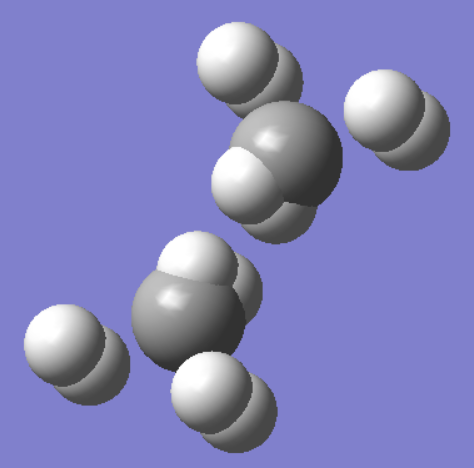
\includegraphics[width=8cm]{long_r_ethene_diagram.png}
\caption{Diagram of pseudo-ethene displaying pseudo-carbon atoms (grey) and \(s\) pseudo-potentials (white).}
\label{fig:long_r_ethene}
\end{figure}

We aim first at reproducing the values for the CH\(^{\bullet}_{3}\) radical as given in Table \ref{table:ch3_s_potentials}. 
This reference CH\(^{\bullet}_{3}\) is created and has its geometry optimised under Hartree-Fock (HF). The pseudo-system is then set up, erasing the hydrogen atoms, setting the carbon charge \(Z_{nucleus} = 1\) and applying \(s\) pseudo-potentials, as well as selecting the correct orbital for the remaining electron. Table \ref{table:ch3_s_potentials} displays some of our results. Promisingly, we are able to produce many sets of potentials that give the correct energy.% with coefficients and exponents of the same order of magnitude as the basis set.

\subsection{Ethene, with \(s\) and \(p\)-potentials}

Next, we take some of these potentials to create a pseudo-ethene system, with the results shown in Table \ref{table:ethene_s_pseudo}. All potentials tested with \(d = 2.0\) a.u. gave results several orders of magnitude away from the reference value. From Figure \ref{fig:long_r_ethene} we may see the reason. One of the potential sets from each carbon is closer to the neighbouring carbon than the neighbour's own potential sets, thus both pseudo-carbons are affected by potentials which do not belong to them. At the shorter range \(d = 0.5\) a.u., the HOMO energy is of the right magnitude, though with errors of \(~ 30\%\). Attempts to eliminate this error lead us to the additional use of the \(p_{z}\) potential \textit{alongside} the \(s\) potentials.

%\begin{table}[ht]
%\caption{Reference values and HOMO-optimised values for Pseudo-ethene using only \(s\)-potentials with an exponent of 10.0}
%\begin{tabular}{c c c}
%\hline
%\multicolumn{3}{c}{Reference} \\
%\hline\hline
%Calculation Type & \multicolumn{2}{c}{C\(_{2}\)H\(_{4}\)\ HOMO )\(\pi\)) energy (eV)} \\
%\hline
%HF & \multicolumn{2}{c}{-10.363} \\
%PBE0 & \multicolumn{2}{c}{-6.632} \\
%\hline
%\multicolumn{3}{c}{Pseudo-system} \\
%\hline\hline
% & \(s\) coefficient & \( \pi \) orbital energy (eV) \\
%\hline
%\multicolumn{3}{c}{d = 2.0 a.u.} \\
%\hline
%HF & -7.521 & -9597.0 \\
%\hline
%\multicolumn{3}{c}{d = 0.5 a.u.} \\
%\hline
%HF & -7.521 & -7.905 \\
%PBE0 & -7.679 & -8.447 \\
%\hline
%\end{tabular}
%\label{table:ethene_s_pseudo}
%\end{table}

\begin{table}[ht]
\caption{HOMO energies for ethene and pseudo-ethene. The pseudo-potentials used in the pseudo-ethene are taken from optimised values for 
pseudo-CH\(^{\bullet}_{3}\) with only \(s\)-potentials and an exponent of 10.0.}
\begin{tabular}{c c c c}
\hline
%\multicolumn{3}{c}{Reference} \\
%\hline\hline
%Calculation Type & \multicolumn{2}{c}{C\(_{2}\)H\(_{4}\)\ HOMO )\(\pi\)) energy (eV)} \\
%\hline
%HF & \multicolumn{2}{c}{-10.363} \\
%PBE0 & \multicolumn{2}{c}{-6.632} \\
%\hline
%\multicolumn{3}{c}{Pseudo-system} \\
%\hline\hline
& $d$ & \(s\) coefficient & \( \pi \) orbital energy (eV) \\
\hline
HF$^a$   &     &        & -10.363 \\
PBE0$^a$ &     &        & -6.632 \\
HF       & 2.0 & -7.521 & -9597.0 \\
HF       & 0.5 & -7.521  & -7.905 \\
PBE0     & 0.5 &-7.678  & -8.447 \\
\hline
\multicolumn{4}{l}{$^a$ All-electron reference values.}\\
\end{tabular}
\label{table:ethene_s_pseudo}
\end{table}

The next step adds a \(p\)-potential centred on the pseudo-carbon, with Table \ref{table:p_potentials} displaying the results. As before, \(d = 0.5\) a.u.. The \(p_{z}\) potential is selected using the procedure described in Section \ref{section:potential_derivation}, with the exponent chosen to give the maximum possible overlap with the \(p_{z}\) orbital, and the matching \(Z_{eff}\) coefficient calculated from the exponent and overlap. The \(s\)-potentials are then optimised once more to give the correct HOMO energy for CH\(^{\bullet}_{3}\). We again take these potentials to create a pseudo-ethene molecule, with the results shown in Table \ref{table:p_potentials}. We can see that these potentials seem to transfer more effectively from the CH\(^{\bullet}_{3}\) system to the ethene, suggesting therefore that whilst the \(s\)-potentials can affect both the \(p_{z}\) and \(\pi\) orbitals, they 
cannot alone describe the relationship between them.

\begin{table}[ht]
\caption{Optimised \(s\)-orbital pseudo-potentials for pseudo-CH\(^{\bullet}_{3}\) and pseudo-ethene. \(d = 0.5\) a.u. The pseudo-ethene is optimised to give the all-electron HOMO reference energies in Table \ref{table:ethene_s_pseudo}.}
\begin{tabular}{c c c c}
\hline
& \(p\) coefficient & \(p\) exponent \\
\hline
\(p_{z}\) potential & -3.267 & 0.295 \\
\hline
Calculation Type & \(s\) coefficient & \(s\) exponent & \(\pi\) \\
\hline\hline
HF & 2.772 & 1.0 & -13.654 \\
 & 6.173 & 5.0 & -14.011 \\
 & 10.381 & 10.0 & -14.061 \\
\hline
PBE0 & 3.483 & 1.0 & -10.325 \\
 & 9.801 & 5.0 & -10.409 \\
 & 18.351 & 10.0 & -12.543 \\
\hline
\end{tabular}
\label{table:p_potentials}
\end{table}

Having successfully created a pseudo-ethene with the correct HOMO, we attempt to have the pseudo-system replicate other properties of the real system:
the singlet-triplet excitation energy ($\Delta_{ST}$) in the $\Delta$SCF framework (energy difference between the triplet and the singlet monoreference
calculations), the ionisation energy (IE) and the energy of the HOMO orbital ($\varepsilon_{HOMO}$). Reference values for the singlet-triplet \(\pi-\pi*\) excitation and first ionisation energies of ethene are given in Table \ref{table:ethene_excitations}. Testing the relevant energies for the optimised pseudo-systems above, we can see from Table \ref{table:ethene_excitations} that the early results are not promising. However, after we abandon the notion of sticking strictly to a \(p_{z}\)-potential exponent that gives the maximum overlap with the real orbital, we discover there is a "sweet spot" of potential coefficients and exponents around which the correct values begin to emerge. Table \ref{table:ethene_excitations} shows our optimal result, chosen to give HOMO, triplet - singlet and ionisation energies closest to the reference values. 

\begin{table}[ht]
\caption{\(s\)-potential fits to ethene properties as defined in the text (eV).}
\begin{tabular}{c c c c c}
\hline
\(s\)-coefficient & \(s\)-exponent & $\Delta_{ST}$  & Triplet - Ion  & $\varepsilon_{HOMO}$  \\
\hline
%\multicolumn{5}{c}{Reference System} \\
%\hline\hline
%& & -3.533 & -9.091 & -10.363 \\
%\hline
%\multicolumn{5}{c}{Pseudo-Systems} \\
%\hline\hline
\multicolumn{2}{c}{\textit{Reference Values}} & -3.533 & -9.091 & -10.363 \\
\hline
&& \multicolumn{3}{l}{\(p\)-coefficient -3.267; \(p\)-exponent 0.295} \\
\hline
0.552 & 0.1 & -3.533 & -27.158 & -27.31 \\
0.608 & 1.0 & -3.533 & -28.247 & -28.395 \\
0.936 & 5.0 & -3.533 & -29.583 & -29.722 \\
\hline
\multicolumn{2}{c}{\textit{Optimal Values}} &\multicolumn{3}{l}{\(p\)-coefficient -3.91; \(p\)-exponent 0.624} \\
\hline
1.5 & 0.5 & -3.533 & -9.806 & -10.062 \\
\hline
\end{tabular}
\label{table:ethene_excitations}
\end{table}

\subsection{C\(\mathbf{_{2n}}\)H\(\mathbf{_{2n+2}}\), \(\mathbf{n=2-12}\)}

\begin{figure}[h]
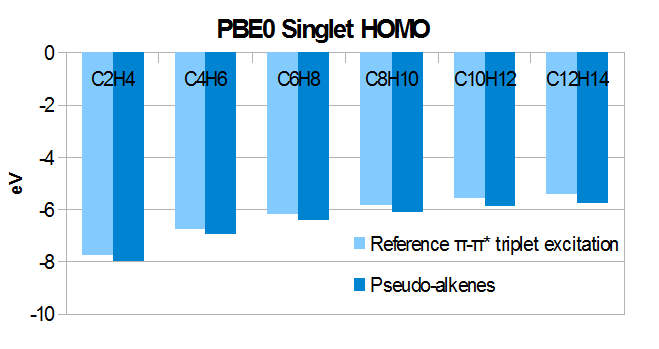
\includegraphics[width=8cm]{pbe0_homo}
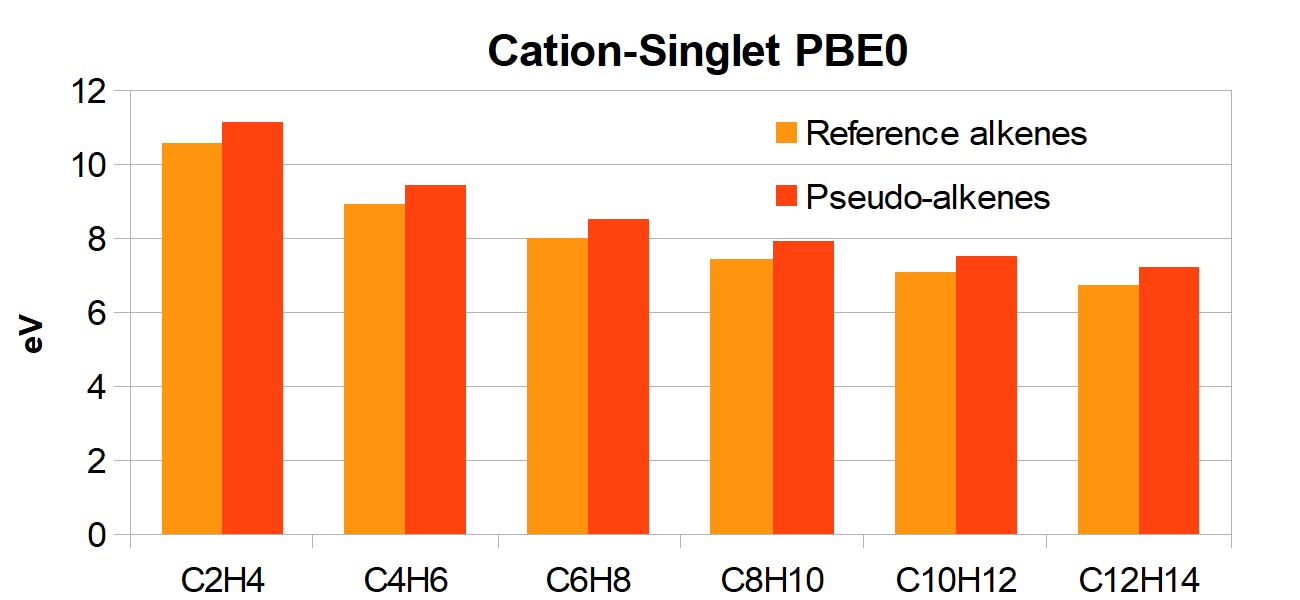
\includegraphics[width=8cm]{pbe0_ionisation}
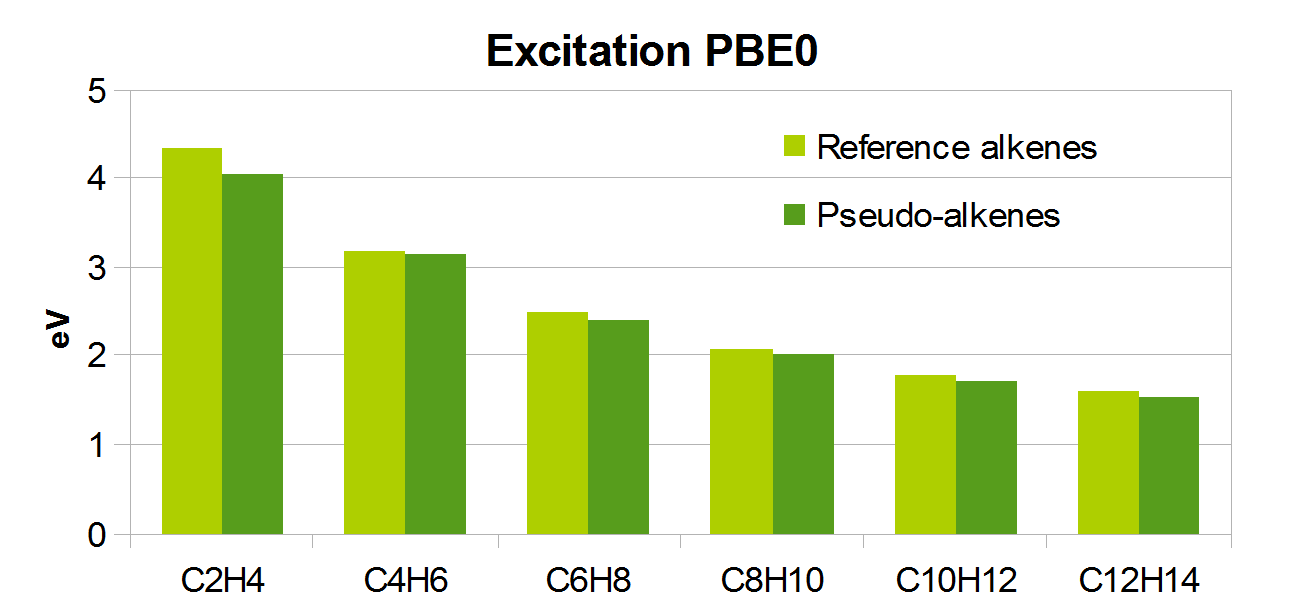
\includegraphics[width=8cm]{pbe0_excitation}
\caption{DFT and TD-DFT (PBE0) comparison of reference and pseudo-system energies across a range of chain alkenes and computational methods.}
\label{fig:alkenes_hf_dft}
\end{figure}
\begin{figure}[h]
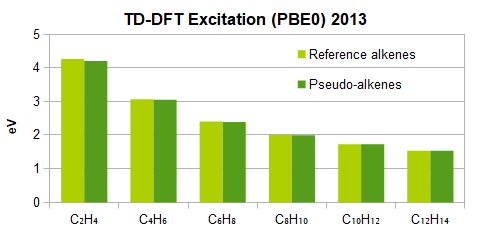
\includegraphics[width=8cm]{tddft_excitation_cd}
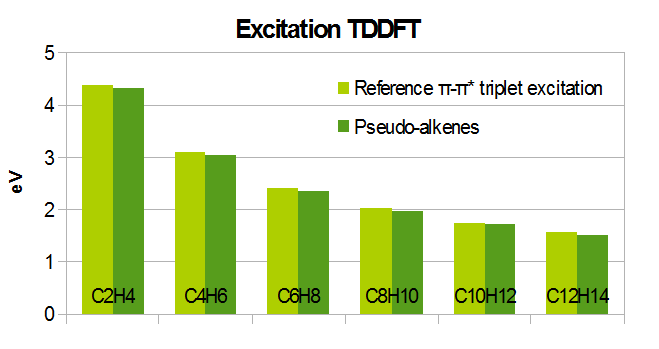
\includegraphics[width=8cm]{tddft_excitation}
\caption{Comparison of pseudo-alkenes with previous\cite{drujon_pseudopotentials_2013} and current potentials using TD-DFT excitation energies.}
\label{fig:alkenes_tddft}
\end{figure}

\begin{table}[h]
\caption{\%-errors across calculation types for short chain alkenes  (C\(_{2}\)-C\(_{12}\))}
\begin{tabular}{c c c c c c }
\hline
Calculation Type & HF & PBE0 & PBE & TPSS & TPSSh \\
\hline\hline
Mean \(\pi - \pi*\) Triplet-Singlet error (\%) & 4.1 & 3.6 & 7.5 & 13.3 & 11.4 \\
Mean Triplet-Ion error (\%) & 5.3 & 6.0 & 8.1 & 10.1 & 9.0 \\
Mean Singlet HOMO error (\%) & 1.3 & 4.0 & 8.5 & 12.0 & 9.7 \\
Mean TD-DFT Excitation error (\%) & - & 2.6 & - & - & - \\ 
\hline
\end{tabular}
\label{table:alkene_errors}
\end{table}

Taking these new potentials we test them against a series of chain alkenes up to length C\(_{12}\), using a variety of functionals. In each case, the geometry of the reference system is optimised according to the method used, 
before taking the reference geometry and applying the pseudo-potentials from Table \ref{table:ethene_excitations}. 
Figures \ref{fig:alkenes_hf_dft} and \ref{fig:alkenes_tddft} show the results. Table \ref{table:alkene_errors} gives a breakdown of the percentage errors for each method across all molecules tested. The pattern of increasing HOMO energy and decreasing cation-singlet and triplet-singlet energies seen in the reference systems is well replicated by the pseudo-alkenes, with the energies following the same gradient.

Also compared are TD-DFT results for this system and results of a previous work of some of the authors, which match to within 3\%.\cite{drujon_pseudopotentials_2013}
Let us recall here that in our previous work potentials were placed at the center of any bond.
%, unlike in our previous work,
%the potentials optimised in this article are fully defined by the position
%of the pseudo-atom: no potentials are placed at the center of any bond.

\subsection{Large Systems}

The potentials derived above are also tested on larger systems.
Figure \ref{fig:rings_graphs} shows the $\Delta_{ST}$, the IE and
HOMO energy values for several ring systems.
As with the short chain alkenes, the general trend of the results is well-replicated
by the pseudo-systems, and the percentage errors, displayed in Table
\ref{table:ring_system_errors}, are similar.

\begin{figure}[h]
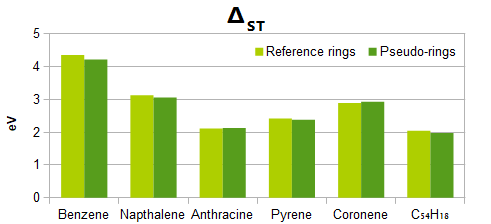
\includegraphics[width=8cm]{ring_pbe0_excitation}
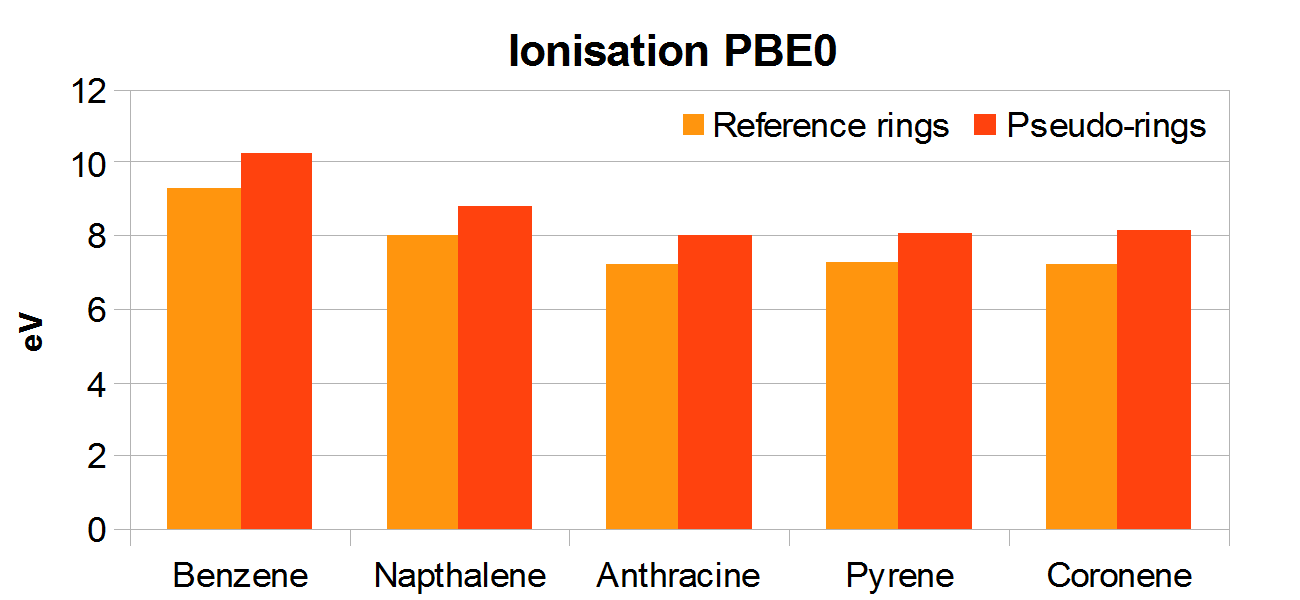
\includegraphics[width=8cm]{ring_pbe0_ionisation}
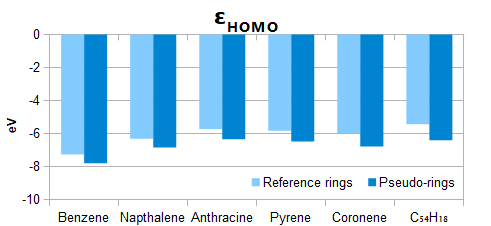
\includegraphics[width=8cm]{ring_pbe0_homo}
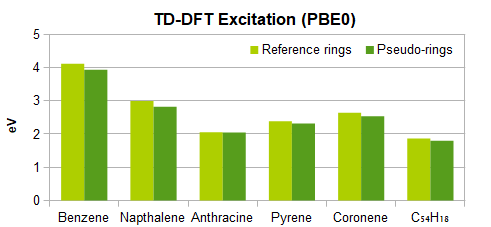
\includegraphics[width=8cm]{ring_tddft_excitation}
\caption{DFT and TD-DFT (PBE0) comparison of reference and pseudo-system energies across a range of ring molecules.}
\label{fig:rings_graphs}
\end{figure}

\begin{figure}[h]
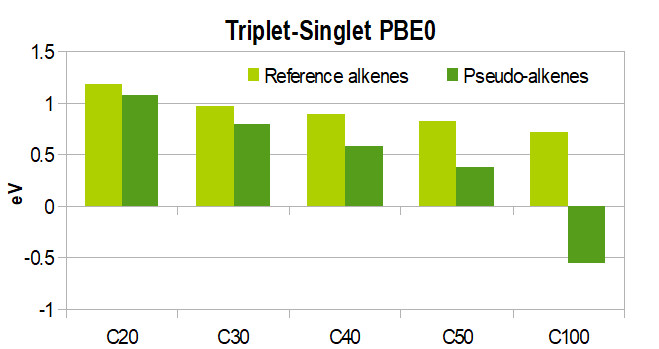
\includegraphics[width=8cm]{pbe0_excitation_long}
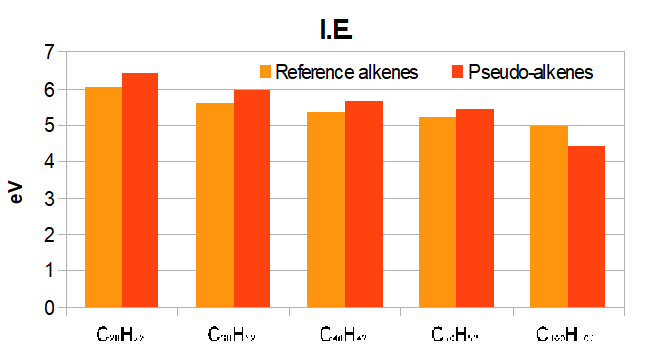
\includegraphics[width=8cm]{pbe0_ionisation_long}
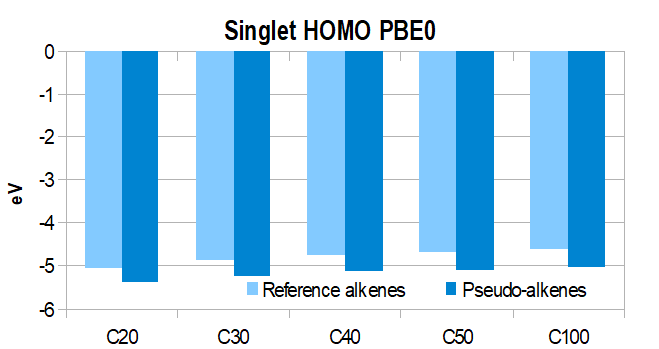
\includegraphics[width=8cm]{pbe0_homo_long}
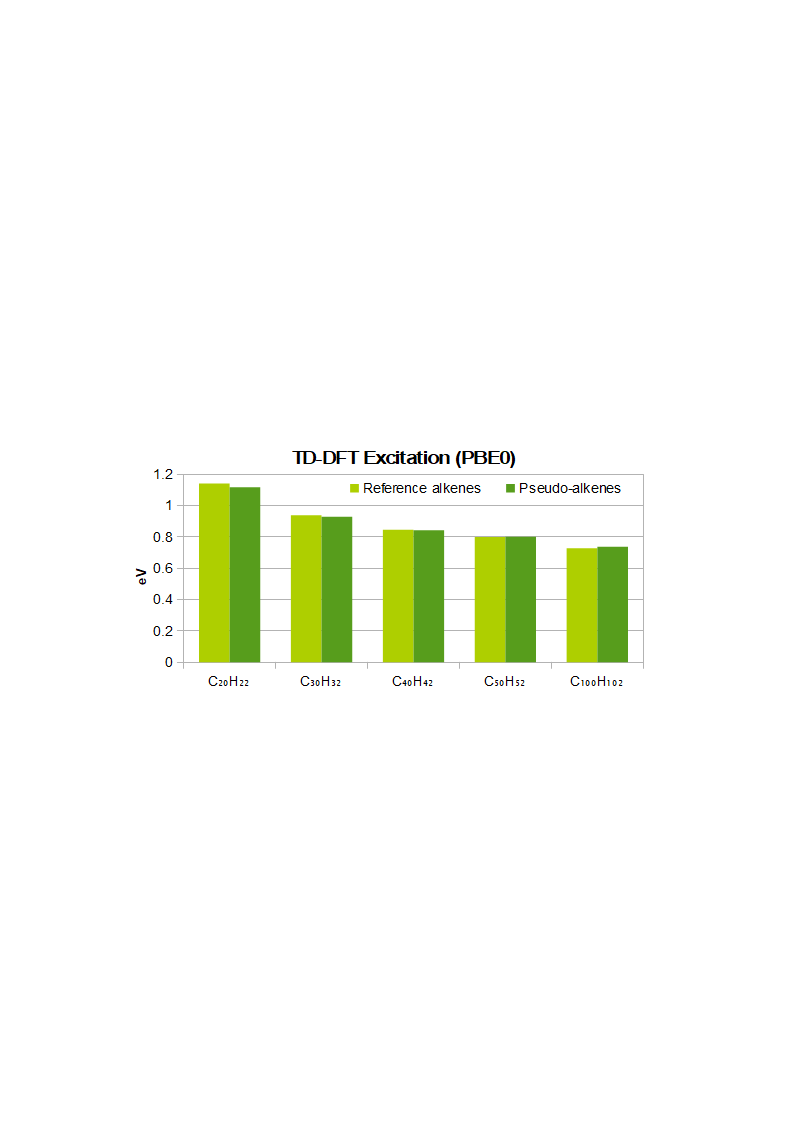
\includegraphics[width=8cm]{tddft_excitation_long}
\caption{DFT and TD-DFT (PBE0) comparison of reference and pseudo-system energies across a range of long chain alkenes (C\(_{20}\)-C\(_{100}\)).}
\label{fig:long_chain_graphs}
\end{figure}

\begin{table}[h]
\caption{\%-errors across calculation types for ring-systems}
\begin{tabular}{c c c c c c }
\hline
Calculation Type & HF & PBE0 & PBE & TPSS & TPSSH \\
\hline\hline
Mean \(\pi - \pi*\) Triplet-Singlet error (\%) & 3.3 & 1.9 & 1.7 & 6.8 & 6.7 \\
Mean Triplet-Ion error (\%) & 7.4 & 10.0 & 12.5 & 14.4 & 13.0 \\
Mean Singlet HOMO error (\%) & 3.4  & 9.3  & 13.4 & 17.1 & 14.7 \\
Mean TD-DFT Excitation error (\%) & - & 0.099 & - & - & - \\ 
\hline
\end{tabular}
\label{table:ring_system_errors}
\end{table}

\begin{table}[h]
\caption{\%-errors across calculation types for long chain alkenes (C\(_{20}\)-C\(_{100}\))}
\begin{tabular}{c c c c c c }
\hline\hline
Calculation Type & HF & PBE0 & PBE & TPSS & TPSSH \\
\hline
Mean \(\pi - \pi*\) Triplet-Singlet error (\%) & 55.3 & 85.8 & 83.4 & 239.8 & 320.2 \\
Mean Triplet-Ion error (\%) & 25.1 & 6.7 & 9.4 & 10.3 & 11.6 \\
Mean Singlet HOMO error (\%) & 1.8 & 7.3 & 11.3 & 16.7 & 13.6 \\
Mean TD-DFT Excitation error (\%) & - & 0.005 & - & - & - \\ 
\hline
\end{tabular}
\label{table:long_alkene_errors}
\end{table}

Figure~\ref{fig:long_chain_graphs} and Table \ref{table:long_alkene_errors} refer to longer 
alkene chains (n up to 100).
The pattern of decreasing ionisation potentials and $\Delta_{ST}$ with increasing HOMO
energy is still followed, with the absolute error remaining consistent.
However, differences in the triplet-singlet energies between the reference and pseudo-systems 
become significant, notably for the largest case.

Unlike for the previous systems, there is a large discrepancy between $\Delta_{ST}$
and TD-DFT results.
This apparent failure of the pseudo-potentials is to be found in the representation
of the triplet state. The expectation values of the $S^2$ operator for the triplet calculations
are plotted in Figure \ref{fig:ssquare}, which shows that the spin contamination
of the triplet state computed as a single configuration (\emph{i.e.} in a SCF
framework) increases in both reference and pseudo-potential cases.
Yet, this effect is strengthened in the pseudo potential calculations.
These results suggest that the triplet state cannot be represented as one configuration
but as a linear combination of monoelectronic excitations as done throught TD-DFT.

In order to show that the recovering of the agreement between the pseudo-potential
and the reference calculations is not an artefact, we give in Table~\ref{tab:coef}
the weight and nature of each excitation (weight larger than 3\%)
in the description of the triplet excited state for
C$_{50}$H$_{52}$ (other values can be found in the SI, which exhibit the same trends).
As can be seen, the agreement is very good. 
%qualitative description of the state is in perfect agreement.
%Numbers differ slightly because the singlet closed shell differs as well between the two calculations.
%Three extra excitations with a weight lower than 3\% appear in the description
%in the pseudopotential calculation.
%Such small numbers are not relevant.

\begin{table}
\caption{\label{tab:coef}Comparison of the weights (all electron \emph{vs.} pseudo-potentials)
of the excitations obtained with TD-DFT
to represent the triplet excited state from the closed shell singlet state.
Example case of C$_{50}$H$_{52}$.}
\begin{tabular}{|l|l|r|r|}
\hline
From    & To       & \multicolumn{2}{c|}{Weight(\%)}\\
MO      & MO       & Ref. & Pseudo.\\\hline\hline
25 a" & 26 a" & 77.0 &   67.1  \\
24 a" & 27 a" & 10.5 &   13.1  \\
23 a" & 28 a" & 3.6  &    5.2  \\\hline
\end{tabular}
\end{table}

\begin{figure}[h]
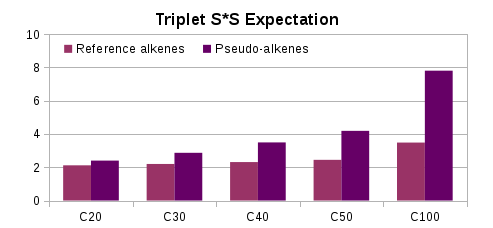
\includegraphics[width=8cm]{ssquare}
\caption{Comparison of $S^2$ expectation values obtained for the calculation
of the first triplet configuration in a SCF formalism, for reference
and pseudo-systems.}
\label{fig:ssquare}
\end{figure}

These results show that the pseudo potentials that we have extracted are able to reproduce the
$\pi$ systems in a variety of situations which are not part of their extraction set.
The molecular orbital virtual space is also well described (cf. Table~\ref{tab:coef}),
which demonstrates that the good agreement with reference calculations is
physically grounded.

\subsection{Computational Details}

Here summarised are details of the methods used in calculation. All Hartree-Fock, DFT and time-dependent DFT (TD-DFT) energy calculations are performed with TURBOMOLE 7.1 \cite{TURBOMOLE}. The basis set used throughout is def-SV(P) \cite{defsvp}. Wherever possible, planar (C\(_{S}\)) symmetry is used. The convergence energy is \(10^{-7}\)H (\texttt{\$scfconv = 7}) for SCF and \(10^{-6}\)H for DFT. When running these calculations the occupation of orbitals is specified manually in the TURBOMOLE control file.

\textbf{Chain Alkenes, Ring Molecules}. In additional to Hartree-Fock calculations, DFT is used with PBE0, PBE, TPSS and TPSSh functionals. \cite{pbe0,pbe,tpss,tpssh} The integration grid size is set at \(m4\). Also used are TD-DFT calculations, where the Tamm-Dancoff approximation (CIS) \cite{tammdancoff} is switched on to avoid triplet instability.

\subsection{Optimisation}

In earlier calculations with only \(s\)-potentials, optimisation was performed by choosing a range of exponent values and attempting to optimise the coefficient at each to produce the HOMO reference energy. Once the \(p_{z}\) potential was added, the \(s\)-potentials were optimised afterward. 

Once we started to look at excitation and ionisation energies however, optimisation became more complicated. Optimisations were at first performed of the s and p-potentials to reach the HOMO energy of ethene as before. With the different potential variables available, we produced a range of optimised potential sets. The best set of these potentials was then chosen and the values altered by hand in order to match as closely as possible three separate reference values: the singlet HOMO energy, the singlet-triplet \(\pi-\pi*\) excitation energy, and the cation-singlet energy. All optimisations used the Brent method in SciPy's optimisation library, with a tolerance of \(1.48*10^{-08}\), and used standard Hartree-Fock calculations.\cite{scipy}

\section{Conclusion}
In this work, we tackled the two main problems of the initial version of our
molecular potentials.
Firstly, the new pseudo potentials for sp$^2$ hybridized
atoms are completely atomic and, even if the directionality of the bonding pattern
has to be fullfilled by correctly postioning the s potentials, no potentials need to
be added relatively to the position of two atoms.
%, \emph{i.e.} potentials
%are to positioned only relatively to the pseudo atom center and not
%relatively to any bond.
Secondly, we gave a physical meaning to all the pseudo potential
terms.
On the contrary of our previous attempt, we do not rely on the "no collapse" term,
which is modeled here by forcing the molecular occupation (\emph{vide infra}).
We could show that not only the occupied orbitals were well reproduced
by use of these new potentials, but also that the virtual space is of good quality
for excited states calculation.

The next steps to be done in the framework of this studies is threefold: the addition of an explicit
"no collapse" term, the reproduction of the gradient through the parametrization
of additional terms and finally the use of such potentials in the framework
of QM/MM calculations as a replacement of hydrogen based link atoms.
The first step is needed in order to avoid to force the molecular orbital occupation and
to avoid spurious virtual orbitals in the active space.
We are confident that the first step could be easily done, as we have already extracted such
terms in the previous version of our potentials.
The reproduction of the gradient is more of a challenge as many electrons were removed from the
system and long range the bielectronic terms shall be very hard to reproduce by monoelectronic
operators.
However, the QM/MM tests shall be quickly started as we could fix the local geometry of the potentials
in the QM part, the MM part would be taken care of without modification of the standard parameters.
%%%%%%%%%%%%%%%%%%%%%%%%%%%%%%%%%%%%%%%%%%%%%%%%%%%%%%%%%%%%%%%%%%%%%
%% The "Acknowledgement" section can be given in all manuscript
%% classes.  This should be given within the "acknowledgement"
%% environment, which will make the correct section or running title.
%%%%%%%%%%%%%%%%%%%%%%%%%%%%%%%%%%%%%%%%%%%%%%%%%%%%%%%%%%%%%%%%%%%%%
\begin{acknowledgement}

The authors thank \ldots

\end{acknowledgement}

- C - H distiance in optimised radical (+optimisation details)

- We are not aiming to exactly reproduce reference values. We aim to give physically relevant effects to the potentials. To go further than huckel or tight-binding models, allowing the study of more than first-neighbour effects. our systems is completely delocalised. (We aren't actually making use of the physical assumptions of the mdoel to probe new systems here, one of the posited potential uses of it). And computational time.

- table 1: some detail of geometry optimisation (and functional / basis set)

- more detail (d) in table 2 title

- line 186 c + D

- some pictures of pseudomolecules

- Review captions (more detail)

- rewrite lambda B lambda bit

- some comments on the increasing error with length of chain. blame alternating bond legth, compare with rings of equal bond length. 

- Triplet - Singlet, not excitation

- Citations at end of sentence? 

- write abstract


%%%%%%%%%%%%%%%%%%%%%%%%%%%%%%%%%%%%%%%%%%%%%%%%%%%%%%%%%%%%%%%%%%%%%
%% The same is true for Supporting Information, which should use the
%% suppinfo environment.
%%%%%%%%%%%%%%%%%%%%%%%%%%%%%%%%%%%%%%%%%%%%%%%%%%%%%%%%%%%%%%%%%%%%%
\begin{suppinfo}

A listing of the contents of each file supplied as Supporting Information
should be included. For instructions on what should be included in the
Supporting Information as well as how to prepare this material for
publications, refer to the journal's Instructions for Authors.

The following files are available free of charge.
\begin{itemize}
  \item Results \& Graphs.ods: Complete results of calculations and associated graphs.
  \item Calculations folder: Contains all calculations used to generate the results in "Results \& Graphs.ods", ordered by molecule
  shape, all-electron/pseudo-molecular calculation and functional/method.
  \item chem\_scripts folder: Contains original scripts used to place and optimise pseudo-potentials.
\end{itemize}

\end{suppinfo}

%%%%%%%%%%%%%%%%%%%%%%%%%%%%%%%%%%%%%%%%%%%%%%%%%%%%%%%%%%%%%%%%%%%%%
%% The appropriate \bibliography command should be placed here.
%% Notice that the class file automatically sets \bibliographystyle
%% and also names the section correctly.
%%%%%%%%%%%%%%%%%%%%%%%%%%%%%%%%%%%%%%%%%%%%%%%%%%%%%%%%%%%%%%%%%%%%%
\bibliography{biblio_pseudo_alex}

\end{document}
